%*************************************************
% A template for PhD and MSc thesis. V1.0.
% Please see "guideline.pdf" first.
%*************************************************
% Iman Izadi, 1394
% Dept. of Electrical and Computer Engineering, IUT
%*************************************************
% این قالب بر اساس "شیوه‌نامه تدوین پایان‌نامه‌ها و رساله‌های 
%تحصیلات تکمیلی" دانشگاه صنعتی اصفهان تهیه شده است
%*************************************************

\documentclass[a4paper,fleqn]{report} 
%\usepackage{refcheck}

% All the packages and general definitions are included in this file: preamble.tex
%*************************************************
% All the packages and definitions are included here.
%*************************************************
%*************************************************
% Iman Izadi, 1394
% Dept. of Electrical and Computer Engineering, IUT
%*************************************************

\usepackage{amsthm,amssymb,amsmath}			% Writing math
\usepackage{epsf,graphicx}									% Including graphics
\usepackage[a4paper]{geometry}							% Fixing page layout and margins
\usepackage{titlesec}											% Change chapter and section titles
\usepackage{setspace}											% Change line spacing
\usepackage[stable,bottom]{footmisc}					% Move footnotes to the bottom of page

\usepackage{zref-perpage}									% Reset footnote counter in each page
\zmakeperpage[1]{footnote}

\usepackage{xepersian}										% Persian
\settextfont{XB Zar}												% Persian font


% Use English digits in equations
\DefaultMathsDigits

% Default footnotes from left to right
\setfootnoteLR

% Use English numbers for English footnotes
\makeatletter
\def\@makeLTRfnmark{\hbox{\@textsuperscript{\latinfont\@thefnmark}}}
\renewcommand\@makefntext[1]{%
    \parindent 1em%
    \noindent
    \hb@xt@1.8em{\hss\if@RTL\@makefnmark\else\@makeLTRfnmark\fi}#1}
\makeatother

% Use dash instead of dot in section numbers
\SepMark{-}										

% Change fonts and margins of section and subsection titles
% For chapters please see firstpages.tex
\titlespacing*{\section}{0pt}{1cm}{0.2cm}
\titleformat{\section}
  {\fontsize{12}{6}\scshape\bfseries}{\thesection}{1em}{}

\titlespacing*{\subsection}{0pt}{.8cm}{0cm}
\titleformat{\subsection}
  {\fontsize{11}{6}\scshape\bfseries}{\thesubsection}{1em}{}
  
% Fix table of contents for chapters
\makeatletter 
\def\@chapter[#1]#2{\ifnum \c@secnumdepth >\m@ne
     \refstepcounter{chapter}%
     \typeout{\@chapapp\space\thechapter.}%
     \addcontentsline{toc}{chapter}%
       	{\@chapapp~\protect\numberline{\tartibi{chapter}\,:\space #1}}
  \else
  	 \addcontentsline{toc}{chapter}{#1}%
  \fi
  \chaptermark{#1}%
  \addtocontents{lof}{\protect\addvspace{10\p@}}%
  \addtocontents{lot}{\protect\addvspace{10\p@}}%
  \@makechapterhead{#2}%
  \@afterheading}
\makeatother
							

\begin{document}

% The first pages (before abstract) are included in this file: firstpages.tex
%*************************************************
% In this file the first few pages are typeset.
% Make the changes accordingly
%*************************************************

% شماره صفحات با حروف
\pagenumbering{adadi}

%***************************
% 1st page: Blank
%***************************
\thispagestyle{empty}
\mbox{}
\pagebreak

%***************************
% 2nd page: Besmelah
%***************************
\thispagestyle{empty}
\begin{center}
	~\vfill
	
\includegraphics[scale=1]{besm1.jpg}
	~\vfill
\end{center}
\pagebreak

%***************************
% 3rd page: Title
%***************************
\thispagestyle{empty}
%\pagenumbering{gobble}
\newgeometry{left=3cm,right=3cm,top=2cm}
\begin{center}

\includegraphics[height=3cm]{iut_logo.png}
\vspace{0.4cm}

\textbf{دانشگاه صنعتی اصفهان}\\
\vspace{0.4cm}

{\large

	دانشکده مهندسی برق و کامپیوتر
}
\vspace{3.5cm}

{\Large
	\textbf{تبدیل خودکار کد ﻣﻨﺒﻊ ﺳﯿﺴﺘﻢ ﻋﺎﻣﻞ از زبان C ﺑﻪ زبان مدلسازی  Promela جهت استفاده برای تست و ارزیابی خودکار مدل}\\
}
\vspace{3.5cm}

{\Large
	پروژه کارشناسی دانشکده کامپیوتر -- نرم افزار\\
}
\vspace{1cm}

{\large
	\textbf{مرضیه علیدادی}\\
}
\vspace{3.5cm}

{\large
	استاد راهنما\\
}
\vspace{0.5cm}

{\large
	\textbf{دکتر الهام محمودزاده}\\
}
\vspace{3.5cm}

\textbf{1400}

\end{center}
\restoregeometry
\pagebreak

%***************************
% 4th page: Signatures
%***************************


%***************************
% 5th page: Acknowledgment
%***************************


%***************************
% 6th page: Rights
%***************************


%***************************
% 7th page: Dedication
%***************************


%***************************
% 8th page: Table of contents   \justifyheading     \centering
%***************************

\titleformat{\chapter}[display]
	{\normalfont\LARGE\bfseries}{\chaptertitlename ~ \tartibi{chapter}}{20pt}{\LARGE}
\newgeometry{left=2.5cm,right=3cm,top=3cm,bottom=2.5cm,includehead=false,headsep=1cm,footnotesep=.5cm}
\baselineskip=.7cm

\addtocontents{toc}{\textbf{\underline{عنوان}}}
\addtocontents{toc}{\hfill\textbf{\underline{صفحه}}\par}
\addcontentsline{toc}{section}{فهرست مطالب}
\tableofcontents
\pagebreak

							

% The abstract of the paper goes here: abstract.tex
%*************************************************
% In this file the abstract is typeset.
% Make changes accordingly.
%*************************************************

\setcounter{page}{1}
\pagenumbering{arabic}						% شماره صفحات با عدد
								

%*****************************************************************
%% تنظیم مناسب صفحه و فونت برای متن اصلی پایان‌نامه
\newgeometry{left=2.5cm,right=3cm,top=3cm,bottom=2.5cm,includehead=false,headsep=1cm,footnotesep=.5cm}
\settextfont{XB Zar}\fontsize{12}{6}\selectfont
\setlatintextfont{Times New Roman}\fontsize{11}{6}
\baselineskip=.9cm

% Moving page number to top right
\pagestyle{myheadings}
%*****************************************************************

% Main chapters
% Chapter 1
\chapter{مقدمه}

در سال‌های اخیر استفاده از انرژی‌های تجدید‌پذیر و جایگزین کردن آن‌ها به جای سوخت‌های فسیلی در کشور‌های توسعه‌یافته و صنعتی با رشد قابل توجهی همراه بوده است. یکی از این انرژی‌های تجدید‌پذیر که بیشتر از سایر انرژی‌ها مورد استفاده قرار گرفته است، انرژی باد است.  توربین‌های بادی طی دو مرحله انرژی باد را به انرژی الکتریکی تبدیل می‌کنند. در مرحله‌ی اول روتور توربین بادی انرژی جنبشی باد را به انرژی مکانیکی تبدیل می‌کند و در مرحله‌ی دوم انرژی مکانیکی توسط ژنراتور به انرژی الکتریکی تبدیل می‌شود. توربین‌های بادی سیستم‌های الکترومکانیکی پیچیده‌ای هستند و از این رو در معرض عیوب\LTRfootnote { Fault } متنوعی در قسمت‌های مختلف همچون سیستم‌ها، محرک‌ها و حس‌گر‌ها قرار می‌گیرند.

از طرف دیگر تشخیص نادرست و دیر‌هنگام این عیوب سبب می‌شود که عیوب در کل سیستم پخش شوند و حتی باعث خرابی\LTRfootnote{ Failure } و از کار‌افتادگی\LTRfootnote{ Downtime } در قسمت‌های مختلف توربین شوند. بنابراین نیازمند مکانیزم کنترلی هستیم که بتواند عیب را در لحظات ابتدایی ظهورش در سیستم شناسایی\LTRfootnote{ Identification } کند و به جبران اثرات منفی عیب بپردازد. از آنجایی که استفاده از توربین‌های بادی در سال‌های اخیر پیشرفت چشمگیری داشته است، بر روی موضوعات مرتبط با توربین‌های بادی کارهای زیادی انجام گرفته است. در زمینه‌ی  آشکارسازی عیوب\LTRfootnote{ Fault Detection } و جداسازی\LTRfootnote{ Fault Isolation } آن‌ها مطالعات زیادی صورت گرفته و روش‌های متعددی ارائه شده است \cite{b6}. همچنین برای جبران اثرات عیب، روش‌های سازش با  عیب\LTRfootnote{  Fault Accomodation  } زیادی پیشنهاد شده‌اند.
\section{پیشینه تحقیق}
 
 \begin{figure}[t]
 \centering
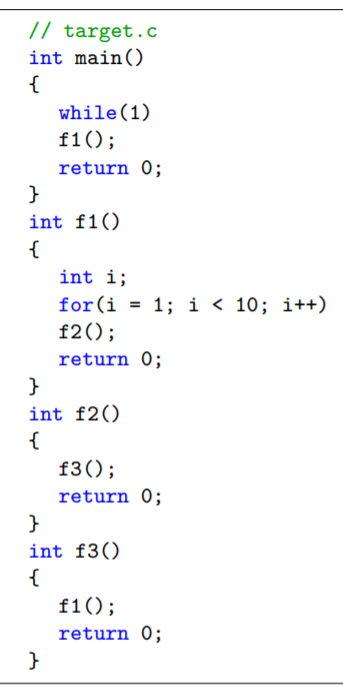
\includegraphics[height=8cm,width=10cm]{b.png}
\caption{ توربین بادی 12 کیلو‌وات (ساخته‌شده به وسیله‌ی چارلز فرانسیس براش) \cite{b1}.}
\label{wt}
\centering
\end{figure}

یک نمونه از توربین‌های بادی اولیه در شکل~\ref{wt} نشان داده شده است. در \cite{a1}، یک مدل معیار\LTRfootnote{ Benchmark Model } برای پیاده‌سازی و مقایسه‌ی روش‌های تشخیص و جداسازی عیب در توربین‌های بادی ارائه شده است. این مدل معیار، یک توربین بادی سه پره‌ی  محور افقی با سرعت متغیر و توان مجاز 4/8 مگا‌وات را که به کنترل گام\LTRfootnote{ Pitch Control }(تغییر زاویه‌ی پره‌‌های توربین بادی حول محور طولی پره‌ها با اعمال فرامین کنترلی) نیز مجهز است، شبیه‌سازی می‌کند. هدف از ارائه‌ی این مدل، بوجود آوردن یک فضای مناسب برای مقایسه و آزمایش روش‌های مختلف تشخیص و جداسازی عیوب بر روی توربین است. از این مدل می‌توان برای مقایسه‌ی روش‌های سازش با عیب که در زمینه‌ی توربین بادی ارائه شده‌اند، استفاده کرد. تعداد زیادی از تحقیقاتی که در سال‌های گذشته در زمینه‌ی تشخیص و جداسازی عیب و همچنین سازش با عیب انجام گرفته است، طرح‌های پیشنهادی خود را بر روی این مدل آزمایش و مقایسه کرده‌اند. 

یکی از اجزای توربین بادی که در معرض عیب قرار دارد، محرک گام پره‌ی توربین می‌باشد. هر یک از پره‌های توربین بادی توسط یک محرک کنترل می‌شوند و با وقوع عیب در  محرک‌ گام هر پره، موقعیت گام آن پره با خطای زیادی مواجه می‌شود. برای حل این مساله،  در \cite{a10} یک روش جبران مبتنی بر تخصیص کنترل\LTRfootnote{ Control Allocation } ارائه شده است. تخصیص کنترل، یکی از رایج‌ترین روش‌های کنترل انعطاف‌پذیر در برابر عیب است. در روش پیشنهادی، گشتاوری که بر اثر عیب یکی از محرک‌ها اتلاف می‌شود، توسط اعمال قانون کنترلی به دو محرک دیگر جبران می‌گردد و توان مطلوب توربین بادی قابل دست‌یابی است.



\section{اهداف و دستاوردهای تحقیق}
از آنجایی که کنترل‌کننده‌ی توربین بادی برای تعیین ناحیه‌ی کنترلی و اعمال دستورات کنترلی مناسب، از اطلاعات حاصل از حس‌گر‌ها استفاده می‌کند؛ وقوع عیب در حس‌گر‌ها می‌تواند سبب تغذیه‌ی اشتباه کنترل‌کننده‌ی توربین شود. در صورتی که کنترل‌کننده‌ی توربین از اطلاعات اشتباه حس‌گر‌ها استفاده کند، دستورات کنترلی که به محرک‌ها اعمال می‌کند اشتباه خواهند بود. این امر سبب می‌شود تا با گذشت زمان، کل سیستم تحت تاثیر قرار گرفته و از حالت بدون عیب فاصله بگیرند. 

در این پایان‌نامه، طرحی پیشنهاد شده است که باعث جلوگیری از کاهش راندمان سیستم، در صورت وجود عیب در حس‌گر‌های اطراف پیشرانه‌ی توربین بادی خواهد شد. در این تحقیق، تشخیص زمان و مکان وقوع عیب، شدت عیب و جداسازی عیب‌ها از یکدیگر به صورت آنلاین مورد بررسی قرار گرفته است. با فرض این که حس‌گر‌های سرعت روتور و ژنراتور و همچنین گشتاور ژنراتور (حس‌گر‌های اطراف پیشرانه‌ی توربین بادی) دچار عیب شوند، با مدل‌سازی مناسب پیشرانه، رویتگر‌هایی را برای تخمین حالت و تولید مانده طراحی کرده و با کمک این رویتگر‌ها (که از نوع رویتگر‌های ورودی ناشناخته هستند)، برای هر یک از حس‌گر‌ها به طور جداگانه سیگنال آشکارسازی عیب تولید می‌کنیم. 

آشکارسازی آنلاین  و سازش با عیوب حس‌گر که در این پایان‌نامه ارائه شده است، بر روی مدل معیار توربین بادی پیاده‌سازی شده و با روش‌های دیگر مورد مقایسه قرار گرفته است. نتایج شبیه‌سازی، بهبود عملکرد سیستم را در صورت بکار‌گیری روش پیشنهادی نشان خواهد داد. 


\section{ساختار پایان‌نامه}
در فصل دوم  به طور مختصر با تاریخچه‌ی انرژی باد آشنا خواهیم شد. همچنین نحوه‌ی عملکرد توربین بادی و اجزای تشکیل‌دهنده‌ی توربین را نیز در این فصل بررسی خواهیم کرد. در پایان این فصل با انواع تقسیم‌بندی‌های توربین‌های بادی از نظر مکان نصب و نحوه‌ی اتصال به شبکه و قرار‌گیری روتور توربین به طور مختصر آشنا خواهیم شد.

در فصل پایانی به بیان نتایج پایان‌نامه و ارائه چند پیشنهاد پرداخته خواهد شد. 


% Chapter 2
\chapter{مفاهیم پایه}

%%%%%%%%%%%%%%%%%%%%%%%%%%%%%%%
%%%%%%%%%%%%%%%%%%%%%%%%%%%%%%%
\section{سیستم‌های هم‌زمان}
همزمانی\LTRfootnote{concurrency} به معنای انجام چند عملیات در یک زمان واحد است. هنگامی که در یک سیستم، چند نخ\LTRfootnote{thread} اجرایی به صورت موازی\LTRfootnote{parallel}  اجرا شوند، همزمانی رخ می‌دهد. هنگامی که همزمانی رخ می‌دهد، ممکن است برای مثال چند نخ اجرایی به صورت همزمان  به یک منبع داده در سیستم دسترسی پیدا کنند. در این صورت، امکان بروز یک سری مشکلات احتمالی وجود دارد. به این دلیل است که به سیستم‌های هم‌زمان\LTRfootnote{concurrent systems} توجه ویژه‌ای می‌شود.

%%%%%%%%%%%%%%%%%%%%%%%%%%%%%%%
\section{سیستم‌های زمان-واقعی}
سیستم‌های زمان-واقعی\LTRfootnote{real-time systems} ، سیستم‎هایی هستند که انجام عملیات و پردازش‌ها توسط آن‌ها باید در کسری از ثانیه رخ‌دهد. این سیستم‌ها محدودیت زمانی مشخصی دارند و باید آن را تضمین کنند. به این ترتیب، یک سیستم زمان-واقعی یا یک عملیات را در آن زمان معین انجام می‌دهد، یا با شکست\LTRfootnote{failure}  مواجه می‌شود.

%%%%%%%%%%%%%%%%%%%%%%%%%%%%%%%%%%%%
\section{Spin}
Spin \cite{1} محبوب ترین ابزار در جهان برای تشخیص نقص های نرم افزاری در طراحی سیستم های همزمان است. با این حال، کد های Promela را به عنوان ورودی در یافت می‌کند و نمی‌تواند برنامه های C را مستقیماً بررسی کند. بنابراین همواره سعی می‌شود تا روش‌هایی واسطه ای برای تبدیل کد C به کد Promela ابداع شود؛ تا امکان توصیف و بررسی کدهای C برای یافتن مشکلات احتمالی در برنامه های همزمان و سیستم های موازی با استفاده از Spin میسر شود.
\\
این ابزار که به صورت متن‌باز\LTRfootnote{open source}  و رایگان دردسترس همه‌ی افراد است؛ قابلیت اجرا برروی سیستم‌عامل‌های Unix ، Linux ، Mac ، Solaris و بسیاری از نسخه‌های Windows را دارد. همچنین، علاوه بر اینکه با کمک خط فرمان\LTRfootnote{command line}  قابل استفاده‌است، دارای یک رابط کاربری گرافیکی کاربرپسند\LTRfootnote{user-friendly GUI}  است، که کار با آن را راحت‌تر می‌کند. در این پژوهش، در چندین مورد، از این ابزار قوی برای وارسی و تایید\LTRfootnote{verification}  مدل‌های Promela استفاده شده‌است. به علاوه، یک راهنمای بسیار کاربردی درباره‌ی نحوه‌ی نصب و اجرای قابلیت‌های مختلف آن دردسترس ‌است.

%%%%%%%%%%%%%%%%%%%%%%%%%%%%%%%%%%%%

\section{زبان Promela}
Promela \cite{4} یک زبان مدل‌سازی فرایند است، که از آن برای تست و وارسی منطق سیستم های موازی استفاده می‌شود. برای وارسی و تایید صحت مدل‌های نوشته شده در این زبان، از ابزار Spin استفاده می‌شود.
\\
این زبان از نظر قواعد نحوی\LTRfootnote{syntactic rules} ، به زبان C شباهت‌ دارد. به همین دلیل است که می‌توان بسیاری از ساختمان‌داده‌های\LTRfootnote{data structures}  معمول و ساده‌ی موجود در زبان C را به طور مستقیم به همان نوع ساختمان‌داده‌ها در Promela ترجمه کرد. از جمله تفاوت‌های موجود در بین این دو زبان، که در این پژوهش نیز مورد بررسی قرار گرفته‌است، عدم وجود توابع \LTRfootnote{functions}  (با همان رفتار مشابه توابع در زبان C ) در زبان Promela است. بنابراین، توابع موجود در زبان C باید به رویه‌ \LTRfootnote{proctype} ها در زبان Promela ترجمه شوند و با استفاده از امکانات دیگری که در این زبان وجود دارد، عملکرد توابع زبان C به خوبی شبیه‌سازی شود. در بخش های آتی، دقیق‌تر به این موضوع پرداخته‌خواهدشد.

%%%%%%%%%%%%%%%%%%%%%%%%%%%%%
\section{زبان \lr{ (Specification and Description Language) SDL}} 
SDL یک زبان مدل‌سازی است که برای توصیف سیستم‌های زمان-واقعی استفاده می‌شود. نمودار SDL فرایند مدل‌سازی را نشان می‌دهد. این زبان می‌تواند به طور گسترده‌ در سیستم‌های خودرو، هوانوردی، ارتباطات، پزشکی و مخابرات استفاده شود.



% Appendices
\appendix
% Appendix 1


% References
\renewcommand{\bibname}{مراجع}
\addcontentsline{toc}{section}{مراجع}

\begin{thebibliography}{99}

\begin{latin}

\baselineskip=.7cm

\bibitem{1}
Spin reference, \textit{https://spinroot.com/spin/Man/README.html}.




\bibitem{2} 
Modex reference, \textit{https://spinroot.com/modex/MANUAL.html}.

\bibitem{3}
K. Havelund and T. Pressburger, \textit{Model checking JAVA programs using
	JAVA PathFinder}, Int. J. Softw. Tools Technol. Transf., vol. 2, no. 4,
pp. 366–381, Apr. 2000.

\bibitem{4} 
Promela reference, \textit{http://spinroot.com/spin/Man/promela.html/}.

\bibitem{5}
B. Vlaovič, A. Vreže and Z. Brezočnik, \textit{Applying Automated Model Extraction for Simulation and Verification of Real-Life SDL Specification With Spin}, in IEEE Access, vol. 5, pp. 5046-5058, 2017, doi: 10.1109/ACCESS.2017.2685238.

\bibitem{6}
K. Jiang, \textit{Model Checking C Programs by Translating C to Promela}, Dissertation, 2009.

\bibitem{7}
H. Mousavi, E. Mahmoudzadeh and A. Ebnenasir, \textit{A Promela Model for Contiki’s Scheduler}, 2020 CSI/CPSSI International Symposium on Real-Time and Embedded Systems and Technologies (RTEST), 2020, pp. 1-10, doi: 10.1109/RTEST49666.2020.9140094.

\end{latin}


\end{thebibliography}

\addcontentsline{toc}{section}{چکیده انگلیسی}
\thispagestyle{empty}

\begin{latin}
\begin{center}

{\Huge Increasing Efficiency in Low-Efficiency Systems}

\vspace{1cm}

{\LARGE{Azin Azadeh}}

\vspace{0.2cm}

{\small azin.azadeh@ec.iut.ac.ir}

\vspace{0.5cm}

March 21, 2015

\vspace{0.5cm}

Department of Electrical and Computer Engineering

\vspace{0.2cm}

Isfahan University of Technology, Isfahan 84156-83111, Iran

\vspace{0.2cm}

Degree: M.Sc. \hspace*{3cm} Language: Farsi

\vspace{1cm}

{\small\textbf{Supervisor: Prof. Bahram Borzou (bahram.borzou@cc.iut.ac.ir)}}
\end{center}
~\vfill



\noindent\textbf{Abstract}

\begin{small}
\baselineskip=0.6cm
In most applications, because of numerous advantages it offers,
digital technology (computer, PLC, microcontroller etc.) is used to
control industrial plants. These types of systems, where the process
under control is continuous-time but the controller is digitally
implemented, are called sampled-data systems. Faults can occur in
sampled-data systems like any other control system. In order to
prevent performance degradation, physical damage or failure, faults
should be promptly detected. In this thesis fault diagnosis in
sampled-data systems is studied. The sampled-data design can be
carried out using direct or indirect design approaches. Direct
design, emphasized in this research, does not involve any
approximations.

Normally, to design a robust fault detection and isolation (FDI)
scheme, a performance index which is a measure of the sensitivity of
the FDI to faults and its robustness to unknown inputs and
disturbances is defined and optimized. Different performance indices
based on norms are considered. Using the direct design
approach and the so-called norm invariant transformation, it is
shown that a sampled-data FDI problem can be converted to an
equivalent discrete-time problem. This will form the foundation of a
unifying framework for optimal sampled-data residual generator
design.

Multirate systems are also abundant in industry. Here, several
methods of residual generation based on multirate sampled data are
developed. The key feature of such residual generators is that they
operate at a fast rate for prompt fault detection. The lifting
technique is used to convert the multirate problem into an
equivalent single-rate discrete-time problem with causality
constraints.

It is generally believed that the optimal multirate design performs
better than the optimal slow-rate and worse than the optimal
fast-rate designs. This conjecture is theoretically proved in this
thesis for general multirate control systems with norms of the
closed-loop system as performance indices. However, it is shown that
the common performance indices in FDI design do not satisfy this
property. To resolve this, an alternative performance index is
defined after formulating the FDI problem as a standard control
problem.

\end{small}

\vspace{0.5 cm}

\noindent \textbf{Key Words}: Fault Detection, Wind Turbine Control, Fault Accomodation, Unknown Input Observers

\end{latin}

%********************************
% Page before last: English Signatures
%********************************
\thispagestyle{empty}
\newgeometry{left=3cm,right=3cm,top=2cm}
\begin{latin}
\begin{center}

\includegraphics[height=3cm]{iut_logo.png}
\vspace{0.4cm}

{\large\textbf{Isfahan University of Technology}}\\

\vspace{0.4cm}
Department of Electrical and Computer Engineering

\vspace{2.5cm}

{\Huge Increasing Efficiency in Low-Efficiency Systems}

\vspace{1.5cm}

{\large
	A Thesis
	
	\vspace{.3cm}
	
	Submitted in partial fulfillment of the requirements
	
	\vspace{.3cm}
	
	for the degree of Master of Science
}

	\vspace{1.5cm}

{\Large
	\textbf{by}
	
	\vspace{.3cm}
	
	\textbf{Azin Azadeh}
}
\end{center}

\vfill

Evaluated and Approved by the Thesis Committee, on March 21, 2015
\vspace{0.5cm}

\begin{enumerate}
\item Bahram Borzou, Prof. (Supervisor)
\vspace{0.5cm}

\item Poorya Parniani, Assoc. Prof. (Advisor)
\vspace{0.5cm}

\item Tahamtan Trabi, Prof. (Examiner)
\vspace{0.5cm}

\item Soraya Sanaei, Assist. Prof (Examiner)
\vspace{0.5cm}

\end{enumerate}

Jamshid Jahangir, Department Graduate Coordinator

\pagebreak
\end{latin}

%***************************
% last page: Blank
%***************************
\thispagestyle{empty}
\mbox{}

% It's finally over. Wasn't that hard, was it?

\end{document}